\chapter{Cơ sở lý thuyết}
\label{chap2}

Hệ thống khuyến nghị là 1 công nghệ hỗ trợ đắc lực cho con người, 
giúp phân tích lượng dữ liệu khổng lồ được cung cấp bởi người dùng. 
Hệ thống dự đoán điểm của các sản phẩm, tạo 1 danh sách sắp xếp thứ các 
sản phẩm này cho mỗi người dùng, và giới thiệu tới người dùng những sản 
phẩm mà họ có thể thích. Nội dung trong phần này trình bày tổng quan về 
hệ khuyến nghị, các mô hình thuật toán cùng với các kỹ thuật thuật khai 
phá dữ liệu trong hệ khuyến nghị hiện có.
\begin{figure}[htbp]
    \centering
    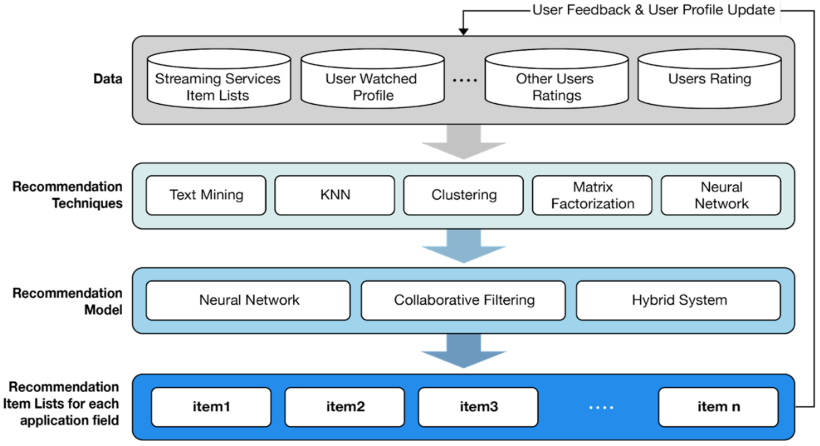
\includegraphics[width=1\textwidth]{imgs/chapter_2/tong-quan-htkn.png}
    \caption{Tổng quan hệ thống khuyến nghị}
    \label{tqhtkn}
\end{figure}
Hình \ref{tqhtkn} là tổng quan 
luồng hoạt động của 1 hệ khuyến nghị, gồm có các bước xử lý: (1) thu 
thập dữ liệu, (2) khai phá dữ liệu, (3) mô hình hóa dữ liệu, (4) và 
đưa ra gợi ý. Dữ liệu sử dụng trong hệ khuyến nghị có thể là các đánh 
giá, bình luận về sản phẩm, danh sách sản phẩm mà người dùng theo dõi, 
v.v. Các kỹ thuật khai phá dữ liệu truyền thống, có thể kể đến như: 
phân cụm, khai phá dữ liệu văn bản, KNN hay là học sâu, sử dụng mạng 
nơ-ron. Tiếp đó, các mô hình khuyến nghị sử dụng các đặc trưng đã 
được trích chọn để có thể mô hình hóa dữ liệu, từ đó đưa ra các khuyến 
nghị phù hợp tới người dùng.

Nội dung trong chương này tập trung giới thiệu và phân loại một cách tổng 
quát về các mô hình khuyến nghị hiện nay, có thể áp dụng vào bất kỳ 1 hệ thống khuyến
nghị nào.

\section{Mô hình khuyến nghị}
Các mô hình khuyến nghị có thể được chia thành 3 nhóm chính \cite{goyani2020review}:
\begin{itemize}
    \item \textbf{Lọc dựa trên nội dung}: Trong cách tiếp cận này, hệ thống sẽ thu thập các dữ
    liệu rõ ràng (điểm đánh giá sản phẩm) hoặc dữ liệu ngầm (bấm vào một đường
    dẫn) và tạo ra hồ sơ người dùng. Hệ thống sẽ thực hiện tư vấn những sản phẩm
    dựa trên những sản phẩm và hành vi liên quan tới hồ sơ người dùng. Do sở thích 
    của người dùng thường được chia thành vài nhóm cơ bản, việc chỉ sử dụng hồ sơ
    của 1 người dùng khiến hệ thống không tận dụng được thông tin từ những người
    dùng khác, từ đó hạn chế sự linh hoạt của hệ tư vấn.

    \item \textbf{Lọc cộng tác}: Không giống với lọc dựa trên nội dung, lọc cộng tác tìm kiếm
    những người dùng có sở thích tương tự nhau. Từ giả định những người dùng A
    có sở thích giống với người dùng B, hệ thống sẽ tiến hành tư vấn cho người dùng
    B những sản phẩm phù hợp người dùng A. Lọc cộng tác có 2 hướng tiếp cận: dựa
    trên bộ nhớ và dựa trên mô hình. Hướng tiếp cận dựa trên bộ nhớ tính toán độ
    tương tự giữa các người dùng từ đó thực hiện tư vấn. Nhược điểm của hướng tiếp
    cận này là sự tốn kém tài nguyên khi số lượng người dùng và sản phẩm tăng lên.
    Hướng tiếp cận dựa trên mô hình sử dụng các mô hình đã được huấn luyện thông
    qua các thuật toán học máy hoặc khai phá dữ liệu để thực hiện tư vấn.

    \item \textbf{Hệ tư vấn lai} Lọc dựa trên nội dung và lọc cộng tác đều có ưu điểm và nhược
    điểm riêng. Để giải quyết vấn đề này, hệ tư vấn lai được sinh ra, là sự kết hợp
    của 2 kỹ thuật trên.
\end{itemize}

Lọc cộng tác là một mô hình lọc thông tin, xây dựng 1 cơ sở dữ liệu sở thích người dùng 
thông qua dữ liệu tưởng tác giữa họ với sản phẩm để dự đoán các sản phẩm phù hợp với sở thích của họ, 
từ đó đưa ra các khuyến nghị về sản phẩm. Ý tưởng của mô hình lọc cộng tác là từ dữ liệu hành vi
tương tác giữa người dùng và sản phẩm, hệ thống sẽ tính toán mức độ tương đồng giữa các người dùng
hoặc giữa các sản phẩm, tạo cơ sở thực hiện khuyến nghị. Những người dùng có mức độ tương đồng cao
sẽ có xu hướng mua những sản phẩm giống nhau. Với mỗi cách tính độ tương đồng sẽ cho một mô hình lọc cộng tác 
khác nhau.

Các mô hình lọc cộng tác có thể được chia ra thông qua 2 hướng tiếp cận: lọc cộng tác dựa trên bộ nhớ và 
lọc cộng tác dựa trên mô hình. Hướng tiếp cận dựa trên bộ nhớ tính toán độ
tương tự giữa các người dùng từ đó thực hiện tư vấn. Nhược điểm của hướng tiếp
cận này là sự tốn kém tài nguyên khi số lượng người dùng và sản phẩm tăng lên. Ngoài ra, hệ 
thống cần tính toán tại thời điểm khuyến nghị, điều này sẽ ảnh hưởng tới thời gian đưa ra dự đoán.
Hướng tiếp cận dựa trên mô hình sử dụng các mô hình đã được huấn luyện thông
qua các thuật toán học máy hoặc khai phá dữ liệu để thực hiện tư vấn. Với hướng tiếp cận này, 
mô hình sẽ cần phải thực hiện huấn luyện trước, nhưng khi thực hiện khuyến nghị sẽ rất nhanh. 
Trong lọc cộng tác dựa trên bộ nhớ, ta có thể phân loại thành: 
lọc cộng tác dựa trên người dùng và lọc cộng tác dựa trên sản phẩm. Lọc cộng tác dựa trên người dùng là 
1 mô hình so sánh sự tương đồng giữa các người dùng thông qua dữ liệu tương tác của họ lên 
các sản phẩm, từ đó khuyến nghị các sản phẩm phù hợp. Lọc cộng tác dựa trên sản phẩm dự 
đoán bằng cách sử dụng độ tương đồng giữa sản phẩm và sản phẩm được chọn bởi người dùng 
thông qua 1 ma trận tương tác của người dùng và sản phẩm. Nói cách khác, lọc cộng tác dựa 
trên bộ nhớ sử dụng các kỹ thuật như: độ tương quan Pearson, độ tương quan cô-sin, KNN 
để tạo các nhóm có đặc tính giống nhau, từ đó khuyến nghị các sản phẩm tới người dùng trong 
nhóm. Do cách hoạt động dựa trên dữ liệu đánh giá, nên mô hình khó có thể hoạt động tốt 
khi không có đủ dữ liệu cần thiết. Để khắc phục vấn đề này, lọc cộng tác dựa trên mô hình 
đưa ra khuyến nghị nhờ sử dụng các thuật toán như: phân cụm, SVD hay PCA.

\subsection{Lọc cộng tác dựa trên bộ nhớ}

\begin{figure}[htbp]
    \centering
    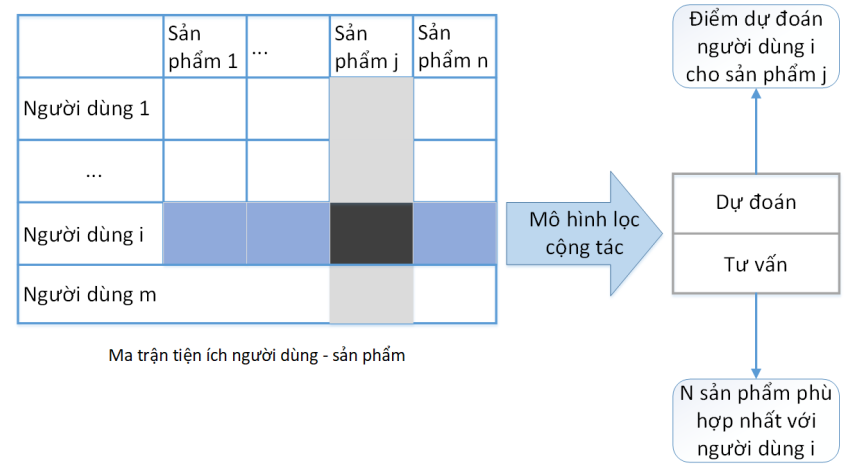
\includegraphics[width=1\textwidth]{imgs/chapter_2/loc-cong-tac.png}
    \caption{Mô hình thuật toán lọc cộng tác}
    \label{lct}
\end{figure}
Thông thường, hồ sơ người dùng – sản phẩm thường được xây dựng từ điểm đánh giá người dùng chấm
cho sản phẩm, được gọi là ma trận tương tác. Ma trận tương tác sẽ có dạng như trong Hình \ref{lct}, với các hàng/cột là danh sách người dùng, cột/hàng là danh sách sản phẩm, các giá
trị trong mỗi ô tương ứng với điểm đánh giá người dùng danh cho sản phẩm. Trong thực
tế, người dùng thường ít đánh giá sản phẩm nên ma trận tiện ích trở nên thưa thớt, nghĩa
là có nhiều giá trị chưa được điền. Hình \ref{lct} là mô hình xử lý, mô tả cho thuật toán lọc
cộng, tác được chia thành 3 bước thực hiện:
\begin{enumerate}
    \item Chuẩn hóa dữ liệu
    \item Tính toán độ tương đồng
    \item Dự đoán mức độ quan tâm của người dùng lên sản phẩm
\end{enumerate}

\subsubsection{Lọc cộng tác dựa trên người dùng}

\underline{Bước 1: Chuẩn hóa dữ liệu}

    Trong thực tế, người dùng “lười” đánh giá sản phẩm khiến ma trận tiện ích trở nên
thưa thớt. Do đó cần chuẩn hóa dữ liệu để loại bỏ những giá trị chưa biết trong ma trận.
Xét ví dụ trong Bảng 1.1 là ma trận tiện ích được xây dựng từ tập người dùng $W = {w_1, ..., w_5}$ và tập sản phẩm $X={x_1, ..., x_5}$. Mỗi sản phẩm được người dùng đánh giá trên thang điểm từ 0 đến 5. Các giá trị “?” nghĩa là người dùng chưa đánh giá những sản phẩm tương ứng.

\begin{table}[h]
\centering
\begin{tabularx}{\textwidth}{|l|>{\centering\arraybackslash}X|>{\centering\arraybackslash}X|>{\centering\arraybackslash}X|>{\centering\arraybackslash}X|>{\centering\arraybackslash}X|}
\hline
      & $x_1$ & $x_2$ & $x_3$ & $x_4$ & $x_5$ \\ \hline
$w_1$ & 5     & 5     & 2     & 0     & ?     \\ \hline
$w_2$ & 2     & 4     & 0     & ?     & ?     \\ \hline
$w_3$ & 0     & 1     & 3     & 4     & 5     \\ \hline
$w_4$ & 5     & ?     & ?     & ?     & 1     \\ \hline
$w_5$ & ?     & ?     & 3     & 2     & 4     \\ \hline
\end{tabularx}
\caption{Ví dụ ma trận tương tác}
\end{table}

    Cách dễ nhất để điền các giá trị còn thiếu vào trong ma trận này là chọn điểm cao nhất
hoặc điểm thấp nhất (5 hoặc 0). Tuy nhiên, khi chọn giá trị này sẽ gây mất cân bằng và
giảm độ chính xác của hệ thống. Một giá trị an toàn có thể điển là điểm trung bình của
thang đo (2,5). Tuy nhiên, giá trị này sẽ không đúng với những người dùng khó tính
hoặc dễ tính. Vì người dùng khó tính sẽ chỉ cho 4 với những sản phẩm họ thích, ngược
lại người dùng dễ tính sẽ cho 1, 2 với những sản phẩm họ không thích. Do đó cần có
một cách chuẩn hóa khác để khắc phục vấn đề này. Các bước chuẩn hóa sẽ được trình bày ngay sau đây. 
\begin{enumerate}
    \item Tính trung bình các điểm đánh giá mà mỗi người dùng đã đưa ra. Ví dụ, người dùng
    $w_1$ đã chấm 4 sản phẩm với số điểm lần lượt là: 5, 5, 2, 0. Như vậy, điểm trung bình người dùng $w_1$ đưa ra là: $\frac{5+5+2+0}{4}=3$.
    \begin{table}[h]
    \centering
    \begin{tabularx}{\textwidth}{|l|>{\centering\arraybackslash}X|>{\centering\arraybackslash}X|>{\centering\arraybackslash}X|>{\centering\arraybackslash}X|>{\centering\arraybackslash}X|
    >{\centering\arraybackslash}X|}
    \hline
          & $x_1$ & $x_2$ & $x_3$ & $x_4$ & $x_5$ & Điểm TB \\ \hline
    $w_1$ & 5     & 5     & 2     & 0     & ?     & 3 \\ \hline
    $w_2$ & 2     & 4     & 0     & ?     & ?     & 2 \\ \hline
    $w_3$ & 0     & 1     & 3     & 4     & 5     & 2.6 \\ \hline
    $w_4$ & 5     & ?     & ?     & ?     & 1     & 3 \\ \hline
    $w_5$ & ?     & ?     & 3     & 2     & 4     & 3 \\ \hline
    \end{tabularx}
    \caption{Ví dụ ma trận tương tác}
    \end{table}

    \item Thực hiện trừ điểm đánh giá của người dùng với điểm đánh giá trung bình của họ
    \begin{table}[h]
    \centering
    \begin{tabularx}{\textwidth}{|l|>{\centering\arraybackslash}X|>{\centering\arraybackslash}X|>{\centering\arraybackslash}X|>{\centering\arraybackslash}X|>{\centering\arraybackslash}X|
    >{\centering\arraybackslash}X|}
    \hline
          & $x_1$ & $x_2$ & $x_3$ & $x_4$ & $x_5$ & Điểm TB \\ \hline
    $w_1$ & 2     & 2     & -1    & -3    & ?     & 3 \\ \hline
    $w_2$ & 0     & 2     & -2    & ?     & ?     & 2 \\ \hline
    $w_3$ & -2.6  & -1.6  & 0.4   & 1.4   & 2.4     & 2.6 \\ \hline
    $w_4$ & 2     & ?     & ?     & ?     & -2     & 3 \\ \hline
    $w_5$ & ?     & ?     & 0     & -1    & 1     & 3 \\ \hline
    \end{tabularx}
    \caption{Ví dụ ma trận tương tác}
    \end{table}

    \item Các ô chưa biết thì điền 0.
    \begin{table}[h]
    \centering
    \begin{tabularx}{\textwidth}{|l|>{\centering\arraybackslash}X|>{\centering\arraybackslash}X|>{\centering\arraybackslash}X|>{\centering\arraybackslash}X|>{\centering\arraybackslash}X|
    >{\centering\arraybackslash}X|}
    \hline
          & $x_1$ & $x_2$ & $x_3$ & $x_4$ & $x_5$ & Điểm TB \\ \hline
    $w_1$ & 2     & 2     & -1    & -3    & 0     & 3 \\ \hline
    $w_2$ & 0     & 2     & -2    & ?     & 0     & 2 \\ \hline
    $w_3$ & -2.6  & -1.6  & 0.4   & 1.4   & 2.4     & 2.6 \\ \hline
    $w_4$ & 2     & 0     & 0     & 0     & -2     & 3 \\ \hline
    $w_5$ & 0     & 0     & 0     & -1    & 1     & 3 \\ \hline
    \end{tabularx}
    \caption{Ví dụ ma trận tương tác}
    \end{table}
\end{enumerate}

Cách chuẩn hóa trên có 2 ưu điểm: (1) Việc trừ đi điểm đánh giá trung bình của người dùng khiến ma trận có giá trị âm, dương. Những giá trị dương ứng với những sản phẩm được người dùng quan tâm
hơn. Những ô có giá trị 0 biểu diễn cho người dùng chưa đánh giá sản phẩm này. Đây là những giá trị cần dự đoán. (2) Số chiều của ma trận tiện ích là rất lớn khi người dùng và sản phẩm tăng lên. Vì vậy, để tiết kiệm bộ nhớ, ma trận tiện ích sẽ được lưu dưới dạng ma trận thưa do những dấu “?” đã được thay bằng giá trị 0.

\underline{Bước 2: Tính toán độ tương đồng và dự đoán}

Với mỗi cách tính độ tương đồng sẽ cho ra một thuật toán lọc cộng tác khác nhau.
Nếu tính độ tương đồng giữa các cặp người dùng ta có thuật toán lọc cộng tác người
dùng. Nếu tính độ tương đồng giữa các cặp sản phẩm, ta có thuật toán lọc cộng tác sản
phẩm. Để tính độ tương đồng giữa người dùng $w_i$ và $w_j$ , ta sử dụng công thức cô-sin:
\begin{equation}
    cosin\_similarity(w_i, w_j) = cos(w_i, w_j)=\frac{w_i^T w_j}{||w_i||_2||w_j||_2}
\end{equation}
Trong đó, $w_i$ và $w_j$ là các véc-tơ tương ứng với hàng/cột $w_i$ và $w_j$ trong ma trận tương tác. Sau khi tính toán được độ tương đồng giữa các cặp người dùng, thuật toán sẽ dự đoán
mức độ quan tâm của người dùng $u$ lên sản phẩm $i$ dựa trên thông tin từ K người dùng
giống $u$ nhất, được định nghĩa theo công thức:
\begin{equation}
    \hat{y}_{i,u}=\frac{\sum_{u, j \in \mathrm{N}(u,i)} \bar{y}_{i, u_j}sim(u, u_j)}{\sum_{u, j \in \mathrm{N}(u,i)}|sim(u,u_j)|}
\end{equation}
Với $N(u,i)$ là tập hợp K người dùng gần giống $u$ nhất và đã đánh giá sản phẩm $i$.

Lọc cộng tác người dùng thường hoạt động không hiệu quả trên các hệ thống lớn do số lượng người dùng khổng lồ. Khi đó, việc tính toán độ tương đồng giữa các cặp người dùng trở nên tốn kém tài nguyên là thời gian.

\subsubsection{Lọc cộng tác dựa trên sản phẩm}
Lọc cộng tác sản phẩm là hướng tiếp cận có thể khắc phục nhược điểm của lọc cộng tác người dùng do số lượng sản phẩm trên hệ thống thường không biến động mạnh. Thay vì tính toán độ tương động giữa các cặp người dùng, lọc cộng tác sản phẩm tính toán độ tương đồng giữa các sản phẩm.

\underline{Chuẩn hóa dữ liệu}
\begin{itemize}
    \item Tính trung bình điểm đánh giá sản phẩm nhận được
    \begin{table}[h]
        \centering
        \begin{tabularx}{\textwidth}{|l|>{\centering\arraybackslash}X|>{\centering\arraybackslash}X|>{\centering\arraybackslash}X|>{\centering\arraybackslash}X|>{\centering\arraybackslash}X|
        >{\centering\arraybackslash}X|}
        \hline
                & $x_1$ & $x_2$ & $x_3$ & $x_4$ & $x_5$ \\ \hline
        $w_1$ & 5     & 5     & 2     & 0     & ?     \\ \hline
        $w_2$ & 2     & 4     & 0     & ?     & ?     \\ \hline
        $w_3$ & 0     & 1     & 3     & 4     & 5     \\ \hline
        $w_4$ & 5     & ?     & ?     & ?     & 1     \\ \hline
        $w_5$ & ?     & ?     & 3     & 2     & 4     \\ \hline
        Điểm TB & 3 & 3.333 & 2 & 2 & 3.333\\ \hline
        \end{tabularx}
        \caption{Ví dụ ma trận tương tác}
    \end{table}

    \item Thực hiện trừ điểm đánh giá của sản phẩm với điểm đánh giá trung bình
    \begin{table}[h]
        \centering
        \begin{tabularx}{\textwidth}{|l|>{\centering\arraybackslash}X|>{\centering\arraybackslash}X|>{\centering\arraybackslash}X|>{\centering\arraybackslash}X|>{\centering\arraybackslash}X|
        >{\centering\arraybackslash}X|}
        \hline
                & $x_1$ & $x_2$ & $x_3$ & $x_4$ & $x_5$ \\ \hline
        $w_1$ & 2     & 1.667 & 0     & -2     & ?       \\ \hline
        $w_2$ & -1    & 0.667 & -2     & ?     & ?      \\ \hline
        $w_3$ & -3    & -2.333& 1     & 2     & 1.667       \\ \hline
        $w_4$ & 2     & ?     & ?     & ?     & -2.333       \\ \hline
        $w_5$ & ?     & ?     & 1     & 0     & 0.667       \\ \hline
        Điểm TB & 3   & 3.333 & 2     & 2     & 3.333   \\ \hline
        \end{tabularx}
        \caption{Ví dụ ma trận tương tác}
    \end{table}

    \item Các ô "?" điền giá trị 0
    \begin{table}[h]
        \centering
        \begin{tabularx}{\textwidth}{|l|>{\centering\arraybackslash}X|>{\centering\arraybackslash}X|>{\centering\arraybackslash}X|>{\centering\arraybackslash}X|>{\centering\arraybackslash}X|
        >{\centering\arraybackslash}X|}
        \hline
                & $x_1$ & $x_2$ & $x_3$ & $x_4$ & $x_5$ \\ \hline
        $w_1$ & 2     & 1.667 & 0     & -2     & 0       \\ \hline
        $w_2$ & -1    & 0.667 & -2     & 0     & 0      \\ \hline
        $w_3$ & -3    & -2.333& 1     & 2     & 1.667       \\ \hline
        $w_4$ & 2     & 0     & 0     & 0     & -2.333       \\ \hline
        $w_5$ & 0     & 0     & 1     & 0     & 0.667       \\ \hline
        Điểm TB & 3   & 3.333 & 2     & 2     & 3.333   \\ \hline
        \end{tabularx}
        \caption{Ví dụ ma trận tương tác}
    \end{table}
\end{itemize}

\underline{Tính toán độ tương đồng và dự đoán}

Dự đoán độ quan tâm của $w_2$ lên $w_5$ sử dụng lọc cộng tác sản phẩm.
\begin{itemize}
    \item Sản phẩm được $w_2$ đánh giá: $\{x_1, x_2, x_3\}$
    \item Độ tương tự giữa $x_5$ và $\{x_1, x_2, x_3\}$ lần lượt là: \{-0.774, -0.449, 0.324\}
    \item Xét K=2, ta có 2 sản phẩm giống $x_5$ nhất : $N(u,i) = \{x_2, x_3\}$ với 
    điểm đánh giá chuẩn hóa là \{0.667, -2\}
    \item $\hat{y}_{(w_2, x_5)}=\frac{0.667*-0.449+(-2)*0.324}{0.324+|-0.449|}=-1.226$
    \item Đưa điểm đánh giá về thang đo ban đầu, ta cộng điểm đánh giá dự đoán với điểm đánh giá
            trung bình của sản phẩm: $-1.226+3.333=2.107$
\end{itemize}

\subsection{Lọc cộng tác phân tích ma trận}
\subsubsection{Giới thiệu}
Ý tưởng chính của phương pháp này là tồn tại các đặc trưng ẩn mô tả sự liên quan
giữa các sản phẩm và người dùng. Ví dụ với các bộ phim, các đặc trưng ẩn có thể rõ 
ràng như: hài, chính kịch, hành động, hoặc chúng là sự kết hợp của các đặc trưng ẩn rõ
ràng, hoặc chúng là những đặc trưng chưa được đặt tên. Tương tự, mỗi người dùng cũng
sẽ có xu hướng thích những đặc trưng ẩn nào đó của phim. Thay vì xây dựng ma trận
của $M$ sản phẩm $X$ một cách độc lập, các đặc trưng ẩn này được huấn luyện đồng thời
với dữ liệu của ma trận $N$ người dùng $Y$.

Với ý tưởng trên, thay vì xây dựng ma trận $Y$ nghĩa là dự đoán các giá trị còn khuyết
trong $Y$ thì thuật toán sẽ cố gắng sấp xỉ ma trận người dùng $W$ và ma trận sản phẩm $X$,
sao cho tích của 2 ma trận này là $\hat{Y}$ xấp xỉ với $Y$.
$$Y \approx \hat{Y} = X^TW$$
\begin{figure}[h]
    \centering
    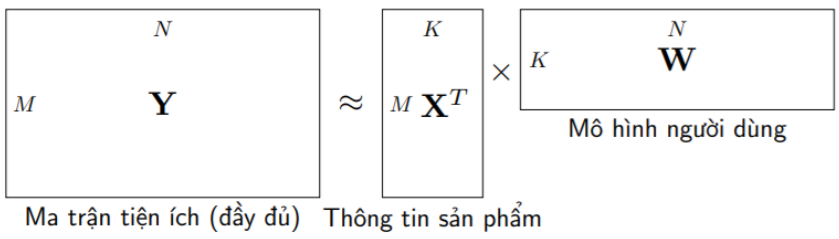
\includegraphics[width=1\linewidth]{imgs//chapter_2/utility_matrix.png}
    \caption{Mô tả phân tích ma trận với K đặc trưng ẩn}
    \label{utility_matrix}
\end{figure}

Hình \ref{utility_matrix} mô tả phương pháp phân tích ma trận tiện ích $Y$ thành 2 ma trận người dùng $W$ và sản phẩm $X$. Trong đó $K$ là số đặc trưng ẩn được giả định của mỗi sản phẩm. Thông thường, $K$ được chọn là một số nhỏ hơn $M$ và $N$ rất nhiều. Khi đó, hạng của $X$ và $Y$ không cao, giúp tiết kiệm tài nguyên.

\subsubsection{Hàm mất mát}
Hàm mất mát được xây dựng dựa trên các ô đã được điền của ma trận $Y$, được định nghĩa như sau:
\begin{equation}
    L(X, W) = \frac{1}{2s}\sum^N_{n=1}\sum_{m:r_{mn}=1}(y_{mn}-x_m w_n)^2+\frac{\lambda}{2}(||X||^2_F + ||W||^2_F)
\end{equation}
Trong đó $r_{mn} = 1$ nếu sản phẩm thứ $m$ đã được đánh giá với người dùng thứ $n$, $||x||^F_2$
là căn bậc 2 của tổng bình phương tất cả các phần tử của ma trận, $s$ là toàn bộ số đánh
giá đã có. Trong công thức trên, thành phần thứ nhất chính là trung bình sai số của mô
hình, thành phần thứ hai là $l2$ regularization, giúp tránh overfitting.

Việc tối ưu cả 2 ma trận $X$ và $W$ cùng lúc là tương đối phức tạp, vì vậy, phương pháp
được sử dụng là tối ưu từng ma trận trong khi ma trận kia cố định đến khi hội tụ.

\subsubsection{Tối ưu hàm mất mát}
Gradient Descent là kỹ thuật được dùng để tối ưu 2 bài toán: cố định $X$ tối ưu $W$ và
cố định $W$ tối ưu $X$. 

Với trường hợp cố định $X$ tối ưu $W$, hàm mất mát được biểu diễn như sau:
\begin{equation}
    L(W)=\frac{1}{2s}\sum^N_{n=1}\sum_{m:r_{mn}=1}(y_{mn}-x_m w_n)^2+\frac{\lambda}{2}||W||^2_F
\end{equation}
Việc tối ưu công thức trên có thể được tách thành N bài toán nhỏ, mỗi bài toán ứng với việc đi tối ưu từng cột của ma trận $W$:
\begin{equation}
    L(w_n)=\frac{1}{2s}\sum_{m:r_{mn}=1}(y_{mn}-x_m w_n)^2+\frac{\lambda}{2}||w_n||^2_2
\end{equation}
Vì biểu thức chỉ phụ thuộc vào các sản phẩm đã được đánh giá bởi người dùng đang xét, công thức có thể được đơn giản bằng cách đặt $\hat{X}_n$ là ma trận được tạo bởi các hàng
tương ứng với các sản phẩm đã được đánh giá đó, và $\hat{y}_n$ là các đánh giá tương ứng. Khi
đó công thức trở thành:
\begin{equation}
    L(w_n)=\frac{1}{2s}||\hat{y}_n - \hat{X}_n w_n||^2 + \frac{\lambda}{2}||w_n||^2_2
\end{equation}
và đạo hàm của nó: 
\begin{equation}
    \frac{\partial L(w_n)}{\partial w_n}=-\frac{1}{s}\hat{X}_n^T(\hat{y}_n-\hat{X}_n w_n)+\lambda w_n
\end{equation}
Từ đó, công thức cập nhật cho mỗi cột của $W$ được định nghĩa như sau:
\begin{equation}
    w_n = w_n - \eta\left(-\frac{1}{s}\hat{X}_n^T(\hat{y}_n-\hat{X}_n w_n)+\lambda w_n\right)
\end{equation}

Khi thực hiện cố định $W$ tối ưu $X$, hàm mất mát được biểu diễn:
\begin{equation}
    L(X)=\frac{1}{2s}\sum^N_{n=1}\sum_{m:r_{mn}=1}(y_{mn}-x_m w_n)^2+\frac{\lambda}{2}||X||^2_F
\end{equation}
Việc tối ưu công thức trên có thể được tách thành $M$ bài toán nhỏ, mỗi bài toán ứng với việc đi tối ưu một cột của ma trận $X$:
\begin{equation}
    L(x_m)=\frac{1}{2s}\sum_{n:r_{mn}=1}(y_{mn}-x_m w_n)^2+\frac{\lambda}{2}||x_m||^2_2
\end{equation}
Vì biểu thức chỉ phụ thuộc vào các sản phẩm đã được đánh giá bởi người dùng đang hàng xét, công thức có thể được đơn giản bằng cách đặt $\hat{W}_m$ là ma trận được tạo bởi các hàng tương ứng với các sản phẩm đã được đánh giá đó, và $\hat{y}_m$ là các đánh giá tương ứng. Khi đó, công thức trở thành:
\begin{equation}
    L(x_m) = \frac{1}{2s}||\hat{y}_m - x_m \hat{W}_m||_2^2 + \frac{\lambda}{2}||x_m||^2_2
\end{equation}
và đạo hàm của nó:
\begin{equation}
    \frac{\partial L(x_m)}{\partial x_m} = -\frac{1}{s}\left(\hat{y}_m-x_m\hat{W}_m\right)\hat{W}^T_m + \lambda x_m
\end{equation}
Từ đó, công thức cập nhật cho mỗi cột của $W$ được định nghĩa như sau:
\begin{equation}
    x_m = x_m - \eta\left(-\frac{1}{s}(\hat{y}_m - x_m\hat{W}_m)\hat{W}_m^T+\lambda x_m\right)
\end{equation}

\section{Phân loại quan điểm người dùng}
\subsection{Tiền xử lý dữ liệu}
Quá trình tiền xử lý dữ liệu gồm 4 bước:(1)Chuẩn hóa văn bản: Bước này, văn bản được đưa về 
chữ thường, các biểu tượng cảm xúc, đường dẫn bị loại bỏ. (2) Tách từ và loại bỏ dấu câu: Tách 
từ là đưa câu bình luận về dạng 1 danh sách các từ cũng với đó là loại bỏ các dấu câu. Các dấu 
câu không có ý nghĩa cho việc phân loại quan điểm. (3) Loại bỏ Stopword: Stopword là những từ 
xuất hiện nhiều nhưng không có ý nghĩa trong quá trình phân loại quan điểm. Ví dụ: “is”, “a”, 
“the”, … (4) Chuyển về dạng chuẩn: Ví dụ: “rooms”=>”room”, “person”=>”people”, các từ được đưa 
về dạng nguyên bản.

\subsection{Trích chọn đặc trưng}
\textbf{TF-IDF}: là một phương pháp thống kê, nhằm phản ánh độ quan trọng của mỗi từ hoặc
1 cụm N-grams đối với văn bản trong phạm vi toàn bộ tài liệu đầu vào. Cho một kho gồm p văn 
bản khác nhau $D={D_1, D_2, ..., D_N}$, mỗi văn bản $D_i$ được tạo bởi các từ $D_i={d_{i1}, ..., 
d_{in}}$. Cho $T={t_1, t_2, ..., t_q}$ là tập hợp những từ xuất hiện trong kho văn bản.
\begin{equation}
    \text{tf-idf}(t_j, D_i) = tf(t_j, D_i)\times idf(t_j, D)
\end{equation}
Trong đó, $tf(t,d)$ của từ $t$ trong văn bản $d$ được định nghĩa theo:
\begin{equation}
    tf(t,d)=\frac{\text{số lần t suất hiện trong d}}{\text{số từ trong d}}
\end{equation}

\textbf{N-grams}: Một cụm N-grams là một dãy gồm N ký tự hoặc từ liên tiếp nhau trong một văn 
bản cho trước. Số phần tử trong một cụm N-grams được gọi là bậc của N-grams. Thông thường, bậc 
của N-grams thường nằm trong khoảng (1,3), với các tên gọi tương ứng là unigram (bậc 1), 
bigram (bậc 2) và trigram (bậc 3). N-grams được dùng để tính tần suất xuất hiện của 1 cụm 
N-grams có trong kho văn bản. Bảng \ref{ngram} là ví dụ biểu diễn N-grams với bậc 1, 2, 3 cho câu: 
“That picture is beautiful.”.
\begin{table}[htbp]
    \centering
    \label{ngram}
    \begin{tabularx}{\textwidth}{|c|X|X|}
        \hline
        Bậc    & Cụm từ                                 \\ \hline
        1 gram & That, picture, is, beautiful           \\ \hline
        2 gram & That picture, picture is, is beautiful \\ \hline
        3 gram & That picture is, picture is beautiful  \\ \hline
    \end{tabularx}
    \caption{Biểu diễn N-grams cho 1 câu}
\end{table}

\subsection{Mô hình học máy có giám sát cho bài toán phân loại quan điểm người dùng}
\textbf{Naive Bayes Classifier}: Bộ phân loại Bayes là một giải thuật thuộc lớp giải thuật phân lớp thống kê, nó có
thể dự đoán xác suất của một phần tử dữ liệu thuộc vào một lớp là bao nhiêu. Bộ phân
loại Bayes được dựa trên định lý Bayes \cite{nam2012nguyen}. Định lý Bayes cho phép tính xác 
suất xảy ra của 1 sự kiện ngẫu nhiên A khi biết sự kiện liên quan B đã xảy ra. Xác suất này được 
ký hiệu là $P(A|B)$, và đọc là "xác suất của A nếu có B". Đại lượng này được gọi là xác suất có 
điều kiện hay xác suất hậu nghiệm vì nó được rút ra từ giá trị được cho của B hoặc phụ thuộc 
vào giá trị nào đó. Theo định lý Bayes, xác suất xảy ra A khi biết B phụ thuộc vào 3 yếu tố:
\begin{itemize}
    \item Xác suất xảy ra A của riêng nó, không quan tâm tới B, ký hiệu là $P(A)$, đọc là xác 
        suất của A. Đây là xác xuất biên duyên hay xác suất tiên nghiệm, nó là “tiên nghiệm” 
        nghĩa rằng nó không quan tâm tới bất cứ thông tin nào của B.
    \item Xác suất xảy ra B của riêng nó, không quan tâm đến A, ký hiệu là $P(B)$ và đọc là 
        "xác suất của B". Đại lượng này còn gọi là hằng số chuẩn hóa (Normalising Constant), vì 
        nó luôn giống nhau, không phụ thuộc vào sự kiện A đang muốn biết.
    \item Xác suất xảy ra B khi biết A xảy ra. Ký hiệu là P(B|A) và đọc là "xác suất của B
    nếu có A". Đại lượng này gọi là khả năng (Likelihood) xảy ra B khi biết A đã xảy ra.
\end{itemize}
Khi đó, xác suất của A khi biết B được định nghĩa bởi công thức:
\begin{equation}
    P(A|B)=\frac{P(B|A)P(A)}{P(B)}
\end{equation}
Từ định lý trên, bộ phân loại Naive Bayes được phát triển và hoạt động như sau \cite{bayes1968naive}:
\begin{enumerate}
    \item Gọi D là tập dữ liệu huấn luyện, trong đó mỗi phần tử dữ liệu X được biểu diễn
        bằng một vector chứa $n$ giá trị thuộc tính $A_1, A_2, ..., A_n$, $X={x_1, x_2, ..., x_n}$
    \item Giả sử có $m$ lớp $C_1, C_2, ..., C_n$, cho 1 phần từ dữ liệu $X$, bộ phân loại sẽ gán 
        nhãn cho $X$ là lớp có xác suất hậu nghiệp lớn nhất. Cụ thể, bộ phân loại Bayes sẽ
        dự đoán $X$ thuộc vào lớp $C_i$ khi và chỉ khi:
        \begin{equation}
            \label{naive_bayes_classifier}
            P(C_i|X) > P(C_j|X) ~~~~ (1\leq i \leq m, i\neq j)
        \end{equation}
    \item Để tìm giá trị xác suất lớn nhất, ta nhận thấy trong công thức \ref{naive_bayes_classifier}
        giá trị $P(X)$ là giống nhau với mọi lớp nên không cần tính. Do đó chỉ cần tìm giá trị lớn 
        nhất của $P(X|C_i)\times P(C_i)$. Trong đó, $P(C_i)$ được ước lượng bằng công thức $P(C_i) = \frac{|D_i|}{D}$ 
        với $D_i$ là tập các phần tử dữ liệu thuộc lớp $C_i$. Nếu xác suất tiền nghiệm $P(C_i)$ cũng không xác định 
        được thì ta coi chúng bằng nhau, khi đó chỉ cần tìm giá trị $P(X|C_i)$ lớn nhất.
    \item Khi số lượng các thuộc tính mô tả dữ liệu là lớn thì chi phí tính toán $P(X|C_i)$ là 
        rất lớn, do đó để làm giảm độ phức tạp, giải thuật Naive Bayes giả thiết các thuộc
        tính là độc lập nhau hay không có sự phụ thuộc nào giữa các thuộc tính. Khi đó
        ta có:
        \begin{equation}
            P(X|C_i) = \prod_{k=1}^n P(x_k|C_i) = P(x_1|C_i)\times P(x_2|C_i) \times ... P(x_n|C_i)
        \end{equation}
\end{enumerate}
Naive Bayes là một giải thuật đơn giản, dễ cài đặt, thời gian huấn luyện nhanh, thực
hiện phân loại khá tốt với các bài toán đa nhãn và không cần quá nhiều dữ liệu huấn
luyện. Tuy nhiên, giả định về sự độc lập giữa các đặc trưng của dữ liệu thường khó xảy
ra trong thế giới thực. Với những đặc điểm trên, Naïve Bayes thường được sử dụng trong
các hệ thống dự đoán thời gian thực, các bài toán dự đoán đa nhãn, phân loại văn bản,
lọc thư rác, …

\textbf{Support Vector Machines}: là kỹ thuật học có giám sát được đề xuất lần đầu
tiên vào năm 1992 cho bài toán phân loại nhị phân \cite{hearst1998support}. Hiện nay thuật toán này được mở
rộng cho các bài toán phân loại đa lớp. SVM hỗ trợ xây dựng một siêu phẳng hoặc một tập hợp các siêu phẳng trong một
không gian nhiều chiều hoặc vô hạn chiều, có thể được sử dụng cho phân loại, hồi quy hoặc các 
nhiệm vụ khác. Để phân loại tốt nhất thì các siêu phẳng nằm càng xa các điểm
dữ liệu của tất cả các lớp (gọi là lề) càng tốt. Trong nhiều trường hợp, không thể phân
chia các lớp dữ liệu một cách tuyến tính trong một không gian ban đầu vì vậy, cần phải
ánh xạ các điểm dữ liệu trong không gian ban đầu vào một không gian mới nhiều chiều
hơn, để việc phân tách chúng trở nên dễ dàng hơn.

Để việc tính toán được hiệu quả, phép ánh xạ sử dụng trong thuật toán SVM chỉ ràng
buộc tích vô hướng của các véc-tơ dữ liệu trong không gian mới có thể được tính dễ
dàng từ các tọa độ trong không gian cũ.
\begin{equation}
    K(a,b)=<a,b>
\end{equation}
Sử dụng hàm đối ngẫu Lagrange, bài toán tìm lệ cực đại của SVM được đưa về bài
toán tìm véc-tơ hệ số $\vec{\alpha}=(\alpha_1, ..., \alpha_n)$ cho phép cực tiểu hóa hàm mục tiêu
\begin{equation}
    W(\vec{\alpha}) = \sum_{i=1}^n \alpha_i - \frac{1}{2}\sum_{i=1}^{n}\sum_{j=1}^{n}y_i y_j \alpha_i \alpha_j K(x_i, x_j)
\end{equation}
đồng thời thỏa mãn:
\begin{equation}
    \sum_{i=1}^{n}y_i \alpha_i = 0 ~~~~~~~ 0\leq\alpha_i\leq C
\end{equation}
Trong đó, $x_i$ và $y_i$ tương ứng là dữ liệu và nhãn của nó, $\alpha_i$ là hệ số cần xác định, 
$C$ là số điểm dữ liệu tối đa được phân loại sai. Quá trình huấn luyện SVM là quá trình xác 
định $\alpha_i$. Phương pháp hiệu quả và thông dụng nhất là tối ưu tuần tự SMO \cite{platt1998sequential}. 
Sau khi phân loại xong, giá trị nhãn phân loại cho mẫu mới được tỉnh bởi:
\begin{equation}
    f(x)=sign(\sum_{i=1}^{n}y_i \alpha_i K(x_i, x) + b )
\end{equation}
với b được tính trong giai đoạn huấn luyện theo công thức:
\begin{equation}
    b=y_i-\sum_{j=1}^{n}y_j \alpha_j K(x_i, x_j)
\end{equation}
Trong đó, $i$ là một hệ số thỏa mãn điều kiện $0<\alpha_i<C$

\textbf{Logistic Regression}: có công thức biểu diễn như sau:
\begin{equation}
    f(x) = \theta(w^T x)
\end{equation}
Trong đó, $f(x)$ là xác suất sinh viên đỗ hay trượt, $x$ là số giờ sinh viên ôn tập, $w^T$ là hằng số 
được huấn luyện sao cho kết quả dự đoán là chính xác nhất, $\theta$ là hàm kính hoạt đưa kết 
quả về dạng xác suất. Tuy nhiên, các bài toán trong thực tế thường có dữ liệu có nhiều đặc 
trưng, cho nên $x=(x_1, x_2, ..., x_n)$ là một véc-tơ, $w$ là ma trận các hằng số. Một số hàm kích hoạt cho mô hình tuyến tính được mô tả trong Hình 2.3. Đường
màu đỏ và vàng không phù hợp với bài toán. Đường màu vàng không bị chặn ở 2 đầu.
Ngoài ra, các điểm dữ liệu trong bài toán không hoàn toàn phân tách nên đường màu đỏ
không phù hợp. Các đường màu xanh lam và xanh lục phù hợp với bài toán của đã nêu
hơn. Chúng có một vài tính chất quan trọng sau:
\begin{itemize}
    \item Là hàm số liên tục nhận giá trị thực, bị chặn trong khoảng (0, 1)
    \item Nếu coi điểm có tung độ là 1/2 làm điểm phân chia thì các điểm càng xa điểm
    này về phía bên trái có giá trị càng gần 0. Ngược lại, các điểm càng xa điểm này
    về phía phải có giá trị càng gần 1. Điều này khớp với nhận xét rằng học càng
    nhiều thì xác suất đỗ càng cao và ngược lại.
    \item Là hàm liên tục nên có đạo hàm mọi nơi.
    \begin{figure}[htbp]
        \centering
        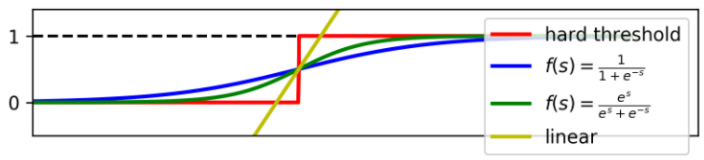
\includegraphics[width=1\linewidth]{imgs//chapter_2/activation_function.png}
        \caption{Một số hàm kích hoạt}
        \label{activation_function}
    \end{figure}
\end{itemize}

Sigmoid là hàm kích hoạt thường xuyên được sử dụng vì nó hoạt động trong khoảng [0, 1]. Hơn nữa, 
đạo hàm của hàm sigmoid rất đơn giản nên được sử dụng rộng rãi.
\begin{equation}
    f(x) = \frac{1}{1+e^{-x}}
\end{equation}
\begin{equation}
    \frac{\partial f(x)}{\partial x} = f(x)(1-f(x))
\end{equation}

Công thức cập nhật cho Logistic Regression sử dụng hàm Sigmoid theo phương pháp Stochastic 
Gradient Descent với điểm dữ liệu $(x_i , y_i)$ là:
\begin{equation}
    w = w +\mu(y_i-z_i)x_i
\end{equation}
Trong đó, $z_i=\theta(w^T x_i)$. Tuy có tên là Regression, nhưng thuật toán này thường sử dụng 
nhiều trong các bài toán phân loại. Mô hình này phân loại dữ liệu dựa trên phương trình siêu 
phẳng $w^T x$ có dạng tuyến tính. Do vậy, mô hình này chỉ phù hợp với các loại dữ liệu mà 2 lớp 
là phân biệt tuyến tính. Logistic Regression không phù hợp với các loại dữ liệu có lớp nằm bên
ngoài đường tròn, lớp nằm trong đường tròn đó. Ngoài ra, các điểm dữ liệu nhiễu sẽ ảnh
hưởng rất nhiều tới độ chính xác của mô hình.

\section{Kết lụân}
Chương 2 đã trình bày các kiến thức, nghiên cứu liên quan về tổng quan mô hình tư vấn và các 
phương pháp trích chọn đặc trưng, phân loại quan điểm người dùng. Chương 3 tiếp theo sẽ trình bày 
về phương pháp đề xuất để giải quyết bài toán đã đặt ra.
